\documentclass[12pt,a4paper]{book}
\usepackage[utf8]{inputenc}
\usepackage{url}

\usepackage{a4wide}
\usepackage{longtable}           % lange Tabellen
%\usepackage[dvips]{epsfig}

\usepackage{fancyhdr}
\pagestyle{fancy}
%\fancyhf{}                              % bisherige Kopf- und Fusszeilen loeschen
\fancyhead[R]{Nico Schottelius}            % rechter Kopfzeileneintrag
%\fancyhead[L]{Projekdokumentation}      % linker Kopfzeileneintrag
%\fancyhead[L]{\thepage}      % linker Kopfzeileneintrag
%\fancyfoot[C]{\thepage}                % Fusszeileneintrag (Seitenzahl zentriert)
\renewcommand{\headrulewidth}{0.4pt}  % Strichstaerke unter der Kopfzeile
% ----------------------------------------------------------------------------
% let's start
\begin{document}
\title{Development of a secure, peer-to-peer, decentralised anonymous chat system}
\date{\today}
\author{Nico Schottelius (nico-hsz-t (o) schottelius.org)}
% ----------------------------------------------------------------------------
\maketitle
\newpage
% ----------------------------------------------------------------------------
% Inhaltsverzeichnis
\tableofcontents
\listoftables
%\listoffigures
\newpage

% ----------------------------------------------------------------------------
% ----------------------------------------------------------------------------
\chapter{Introduction}

Anonymous communication networks were first intro-
duced by David Chaum in his seminal paper [10] describing
the mix as a fundamental building block for anonymity.
(aus tor2)

\subsection{Abstract}
hier oder weiter oben? - siehe lisa vortrag!

\subsection{Abbreviations}
\subsection{Starting Position}
local, skype, untrustworthy

\subsection{Motivation}
From EBS + EOF

\subsection{Objectives}
From EOF + Latency "`low"', eventual consistency
\subsubsection{Steganographic}
Not for hiding, but to support longer überleben?
http is pretty well suited for this.
mixing with smtp, imap, pop3, tcp. etc.



% ----------------------------------------------------------------------------
\chapter{Analysis and Comparision of Chat Systems}

    1. Detailed analysis and comparison of open and legacy chat systems
        to summarise current chat system features and their
        security characteristics.


% ----------------------------------------------------------------------------
\section{IRC}
\subsection{History}

Since 1989 deleoped\ref{rfc2810},
first formally documented in May 1993 by RFC 1459\ref{rfc1459}.

\begin{quote}
All client-to-server IRC protocols in use today are descended from the protocol implemented in the irc2.4.0 version of the IRC2 server, and documented in RFC 1459. Since RFC 1459 was published, the new features in the irc2.10 implementation led to the publication of several revised protocol documents (RFC 2810, RFC 2811, RFC 2812 and RFC 2813); however, these protocol changes have not been widely adopted among other implementations.\ref{irc-wp}
\end{quote}

% ----------------------------------------------------------------------------
\subsection{Architecture}
central server, server network
IRC, the \textit{Internet Relay Chat}, has been developed since 1989
and is defined in severals Internet RFCs.\footnote{See \cite{rfc1459}, 
\cite{rfc2810}, \cite{rfc2812} and \cite{rfc2813}.}
IRC networks consist of IRC servers and IRC clients:

\begin{verbatim}
                       1--\
                           A        D---4
                       2--/ \      /
                             B----C
                            /      \
                           3        E

   Servers: A, B, C, D, E         Clients: 1, 2, 3, 4

                    [ Fig. 1. Sample small IRC network ]

\end{verbatim}\footnote{Source: \cite{rfc2810}}
IRC is organised centrally, as stated in \cite{rfc2810}:
\begin{quote}
The IRC protocol provides no mean for two clients to directly
communicate.  All communication between clients is relayed by the
server(s).
\end{quote}

There is, however, an unstandartised client extension named 
\textit{Direct Client-to-Client} (DCC) available in most IRC clients
that enables direct connections.\footnote{See \cite{dcc}, \cite{dcc2}.}

% ----------------------------------------------------------------------------
\subsection{Security}
SSL is being used in some networks, but not standartised. [nico]
optional encryption.
% ----------------------------------------------------------------------------
\section{Silc}
SILC Project develops the Secure Internet Live Conferencing protocol (SILC),
\url{http://silcnet.org/general/}
\url{http://silcnet.org/support/documentation/specs/}

central
\url{http://silcnet.org/support/documentation/wp/silc_protocol.php}


% ----------------------------------------------------------------------------
\section{Skype}
More VoIP
% ----------------------------------------------------------------------------
\section{MSN}
More VoIP
% ----------------------------------------------------------------------------
\section{ICQ}
More VoIP


% ----------------------------------------------------------------------------
\section{Security features and Comparision}

\begin{longtable}{|c|c|c|}
\caption{Chat system comparision with security features}\\
\hline
\textbf{Name} & \textbf{IRC} & \textbf{SILC}\\
\hline
\textbf{Single point of attack} & yes & yes\\
\hline
\textbf{Encrypted traffic} & optional & yes\\
\hline
\end{longtable}

All the solutions with objectives.

\chapter{Analysis of features and security requirements}
\label{requirements}
% -----------------------------------------------------------------------------
From the previous analysis of chat systems and related communication protocols,
several drawbacks can be seen. Most systems suffer a single point of failure,
which is due to the central architecture. Further the message content is often
neither protected nor verified.

The following security features are derived from the weaknesses of the previously
analysed systems as well from the thesis objectives.
% -----------------------------------------------------------------------------
\section{Anonymity}
One of the main objectives of this thesis is to provide a chat system that
hides who is talking to whom. If an attacker controls all hosts that are
part of the chat network, it is impossible to guarantee anonymity.

Thus the implementation should support be resistent against a high percentage
of attacker nodes in the network.
% -----------------------------------------------------------------------------
\subsection{Sender to receiver anonymity}
Providing anonymity of two people talking to each other is \textbf{not} 
required due to the objectives of this thesis.
% Nico: 1 => reformulate
% -----------------------------------------------------------------------------
\subsection{Receiver identification}
The receiver should be able to verify the identity of the sender, so she
can be sure that the message originated from the correct person.
% Nico: 1 => reformulate
% -----------------------------------------------------------------------------
\section{Confidentiality}
The content of the conversations should be hidden from eavesdropper.
Being able to read the content of messages may also reveal the identity
of the chat partners and thus the anonymity would vanish.
% Nico: 1 => reformulate

% FIXME: solution:
% We encrypt every message via public-key cryptography\cite{pgp-1},
% so that only the receiver can decrypt and view the message content.
% 
% -----------------------------------------------------------------------------
\section{Integrity}
As messages may contain important content, it is necessary that the integrity
is guaranteed.
% Nico: 1 => reformulate
% -----------------------------------------------------------------------------
\section{Availability}
Most traditional systems rely on central infrastructure to operate, in which a
single party (like the operator) can disable the service. 
No service can be run reliable, if an attacker with infinite resources is assumed.
Thus the requirement for this chat system is to survive the attack of a single
party and to continue delivering the chat service.
% Nico: 1
% -----------------------------------------------------------------------------
\section{Reliable against single user attacks}
Traditional chat networks depend on one or more central organised servers.
An attacker can stop all communication, if she runs a successful denial
of service ("`DoS"') attack against the central systems.
To protect against this, EOF uses a dynamic peer-to-peer network, which works
as long as the minimun number of peers and the destination peer is available.
It has no dependency on a central server.
% Nico: 1.0
% -----------------------------------------------------------------------------
\section{Hide packets in network stream}
As said before, we don't think it's possible to hide the participation in the
chat network. To be able to send packets, although an attacker \emph{knows}
about the participation, EOF embeds all chat packets into other (well known)
protocols (which is knows as steganography\cite{stegano-1}).
EOF does not implement nor specify \emph{transport protocols} itself.
The EOF community is urged to implement them in a creative way: Usage
of well-known protocols like TCP\cite{tcp-1}, HTTP\cite{http-1},
SMTP\cite{smtp-1} or even transmission of packets on avian
carriers\cite{avian-1} are encouraged. The tunneling of EOF packets through
those protocols (also know as obfuscation) makes it harder to detect
and \emph{block} EOF traffic.
If an attacker wants you to stop sending messages, she has to completly
remove you from the network, because any open protocol may be (ab)used to
encapsulate EOF packets into it.
% Nico: 1.0
% -----------------------------------------------------------------------------
\section{Non security related features}
To be able to be compete with other chat protocols, EOF needs
to support \emph{direct} and \emph{group chat}, which is
implemented by two different chat destinations:
\begin{enumerate}
\item \emph{Peers}
\item \emph{Groups of peers}
\end{enumerate}
A peer is just another person (direct chat), a group of peers is the EOF
equivalent of the IRC channel\cite{irc-1}. As there is no central server,
groups of peers are managed by each client, and thus the compositions of
group members may be different on different peers.
-- 
Additionally, for practical reasons, EOF must support the following
chat features:
\begin{enumerate}
\item Direct chat ("`message is only seen by one person"')
\item Group chat ("`message is sent to specific group, which may consist of
more than one person"')
\end{enumerate}

% -----------------------------------------------------------------------------
\section{Summary}
\begin{enumerate}
\item Nobody, but the intended receiver(s) know(s) \emph{that} you wrote a message.
\item Nobody, but the intended receiver(s) can view the \emph{message content}.
\item Nobody, but the intended receiver(s) can \emph{verify} the source of the message being you.
\item Nobody, but the intended receiver(s) know(s) \emph{who} you sent a message to.
\item The network must survive attacks of a single attacker.
\item Hard (if not practilcally impossible) to block chatting.
\end{enumerate}



\chapter{Analysis of related communication protocols}

% ----------------------------------------------------------------------------
\section{Mix networks}
Mix networks are also known as onion routing or digital mixes and
were invented by David Chaum in 1981.\cite{Chaum:1981:UEM:358549.358563}
\begin{figure}
    \centering
    \caption[Mixes: Packet Flow]{Mixes: Packet Flow\\Image source \url{http://upload.wikimedia.org/wikipedia/en/2/23/Decryption_mix_net.png}}
    \label{mixesflow}
    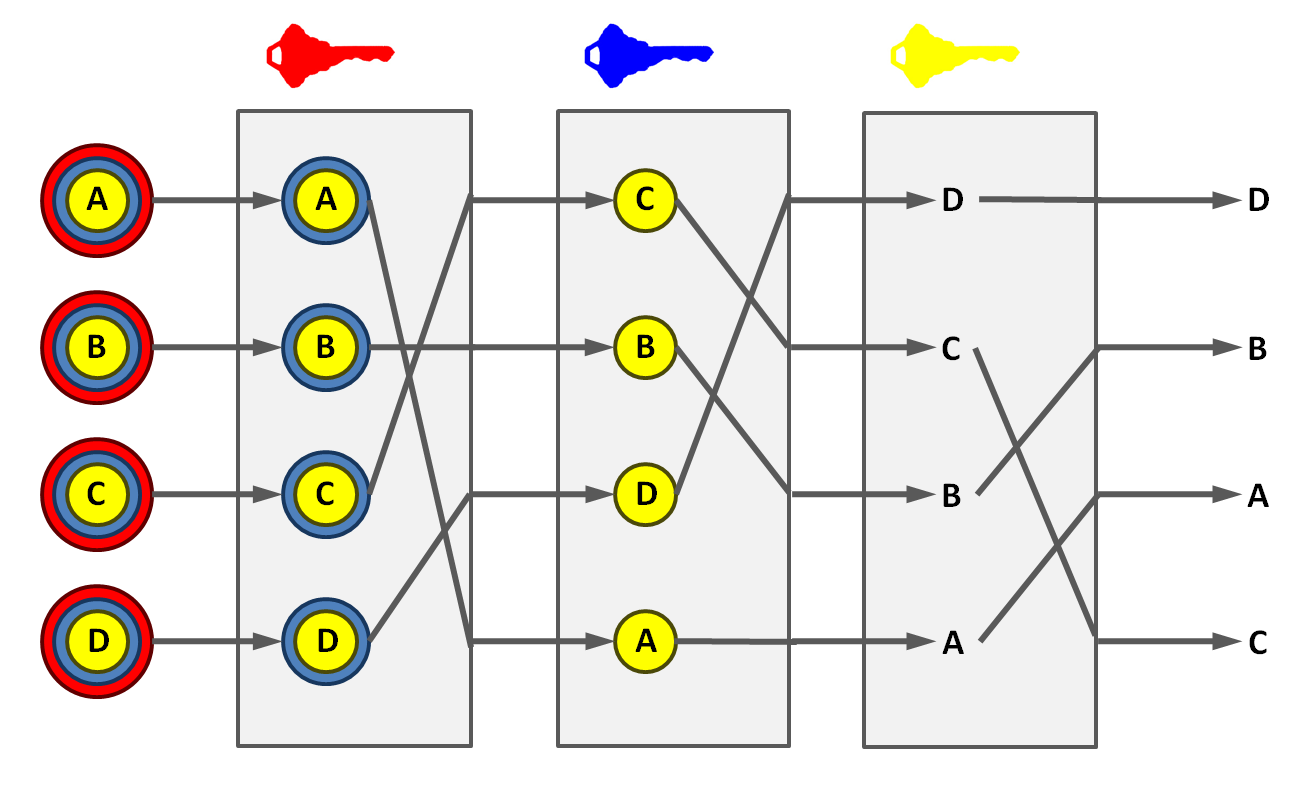
\includegraphics[scale=0.3]{Decryption_mix_net.png}
\end{figure}
The base of Mixes is the multiple encrypted packet that is send through a
number of peers (the mixes) as shown in figure \ref{mixesflow}.
Every peer decrypts the message, which reveals which is the next peer
to send the packet to. Using this method, every peer only knows about
its predecessor and successor. For encryption Public-Key-Cryptography (RSA) is used.
The original approach was focussing on Mixes for e-mail delivery.
% Patent \url{http://patft1.uspto.gov/netacgi/nph-Parser?Sect1=PTO2&Sect2=HITOFF&p=1&u=%2Fnetahtml%2FPTO%2Fsearch-bool.html&r=1&f=G&l=50&co1=AND&d=PTXT&s1=6266704.PN.&OS=PN/6266704&RS=PN/6266704}
% ----------------------------------------------------------------------------
\section{Tor}
The Tor network has been published in 2004
at the 13th USENIX Security Symposium by Roger Dingledine, 
Nick Mathewson and Paul Syverson.\cite{tor}
The idea behind Tor is to provide a general purpose, 
low latency anonymising network stack.
They explicitly do not include application level anonymity
(like stripping user agent information from a http request) and
reason this to leave it up specialised projects.
Tor does (by design) offer no protection against end-to-end attacks
(for instance using traffic analysis) to support low latency applications.
The Tor software provides access to its network via
a SOCKS proxy interface.
Tor does not use the traditional mix approach:
\begin{quote}
Rather than using a single multiply encrypted
data structure (an onion) to lay each circuit, Tor now uses an
incremental or telescoping path-building design, where the
initiator negotiates session keys with each successive hop in
the circuit.\footnote{Quote from \cite{tor}.}
\end{quote}
%\url{http://en.wikipedia.org/wiki/Onion_routing}
% Reply onions have been replaced by a rendezvous system, 
%Generic transport protocol.
%    Separation of “protocol cleaning” from anonymity:

%Onion Routing originally required a separate “application
%proxy” for each supported application protocol—most of
%which were never written, so many applications were never
%supported.
%Tor uses the standard and near-ubiquitous
%SOCKS proxy interface, allowing us to support most
%TCP-based programs without modification. Tor now relies on
%the filtering features of privacy-enhancing application-level
%proxies such as Privoxy [39], without trying to duplicate those
%features itself.
%% No mixing, padding, or traffic shaping (yet): Onion
%% Routing originally called for batching and reordering cells
%% as they arrived, assumed padding between ORs, and in later
%% designs added padding between onion proxie
%% 
%% 
%% Perfect forward secrecy: In the original Onion Routing
%% design, a single hostile node could record traffic and later
%% 
%% ...
%% 
%% 
%% Not secure against end-to-end attacks: Tor does not
%% claim to completely solve end-to-end timing or intersection
%% attacks. Some approaches, such as having users run their own
%% onion routers, may help; see Section 9 for more discussion.
%% 
%% \cite{tor}
% ----------------------------------------------------------------------------
\section{Off-the-Record Messaging (OTR)}
Off-the-Record Messaging (OTR) has been introduced by
Nikita Borisov, Ian Goldberg and Eric Brewer in 2004.\cite{otr}
In contrast to other approaches OTR does not rely on long term
keys as usually used in Public-Key-Cryptography. OTR instead
uses short time keys, to prevent decryption of sniffed messages,
if access to the private key is gained after some time.

Furthermore OTR includes measures to include repudiability, though
provide authentication during a session using
message authentication codes (MAC).
OTR works as a drop in for existing chat programs and offers auto-detection
if the other side is capable of using OTR as well.
%As of OTR 3.1 the protocol supports mutual authentication of users using a shared secret through the socialist millionaire protocol. This feature makes it possible for users to verify the identity of the remote party and avoid a man in the middle attack without the inconvenience of manually comparing public key fingerprints through an outside channel. 
% \url{http://de.wikipedia.org/wiki/Off-the-Record_Messaging}
% ----------------------------------------------------------------------------
\section{Freenet}
Freenet has been published in 2001 by
Ian Clarke , Oskar Sandberg , Brandon Wiley and Theodore W. Hong.\cite{freenet}
Its primary use the anonymous storage (and retrieval) of files.
Freenet is described as follwing:
\begin{quote}
Freenet is free software which lets you anonymously share files, browse and publish "freesites" (web sites accessible only through Freenet) and chat on forums, without fear of censorship. Freenet is decentralised to make it less vulnerable to attack, and if used in "darknet" mode, where users only connect to their friends, is very difficult to detect.\footnote{Quote from \url{https://freenetproject.org/whatis.html}}
\end{quote}
% ----------------------------------------------------------------------------
\section{I2P}
The I2P project, originally Invisible Internet Project, is supposed to be
"`a scalable framework for anonymous communication"'.\cite{i2p} 
It is described on the website as following:
\begin{quote}
I2P initially began in Feb 2003 as a proposed modification to Freenet to allow it to use alternate transports, such as JMS, then grew into its own as an 'anonCommFramework' in April 2003, turning into I2P in July, with code being written in earnest starting in August '03. I2P is currently under development, 
following the roadmap.\footnote{Quote from \url{http://www.i2p2.de/how_intro}.}
\\
...
\\
I2P is a scalable, self organizing, resilient packet switched anonymous network layer, upon which any number of different anonymity or security conscious applications can operate. Each of these applications may make their own anonymity, latency, and throughput tradeoffs without worrying about the proper implementation of a free route mixnet, allowing them to blend their activity with the larger anonymity set of users already running on top of I2P.\footnote{Quote from \url{http://www.i2p2.de/techintro.html}.}
\end{quote}
Although the overall of the impression of the website indicates that it may provide a
reasonable base for anonymous communications, the lack of a central architecture or
design paper makes it hard to judge about it.
%% I2P (initially short for Invisible Internet Project)
%% 
%% I2P is an anonymizing network, offering a simple layer that identity-sensitive applications can use to securely communicate. All data is wrapped with several layers of encryption, and the network is both distributed and dynamic, with no trusted parties.
%% 
%% Many applications are available that interface with I2P, including mail, peer-peer, IRC chat, and others.
%% 
%% 
%%  a low latency, fully distributed, autonomous, scalable, anonymous, resilient, and secure network
%% 
%%   I2P is a low latency mix network, 
%% 
%% 
%% \url{http://en.wikipedia.org/wiki/I2P}
%% 
%% \url{http://www.i2p2.de/_static/images/endToEndEncryption.png}
%% 
%% The first time a client wants to contact another client, they make a query against the fully distributed "network database" - a custom structured distributed hash table (DHT) based off the Kademlia algorithm. This is done to find the other client's inbound tunnels efficiently, but subsequent messages between them usually includes that data so no further network database lookups are required.
%% 
%% This "garlic encryption" lets Alice's router wrap up multiple messages into a single "garlic message",
% ----------------------------------------------------------------------------
\section{RUDP}

packet loss: ja
Packet duplicates:
Out of order packets: don't care - no fragmentation
    - probably missing conversation!
    Bit errors: not applicable
    Delay of packets: upper limit (?) 


    - verschieden kaäle:
        - email = sticky, cached, slow
            - tcp = fast, temporarily

            - rudp:
                http://www.javvin.com/protocolRUDP.html
                        rfc908, rfc1151

TCP Reliable transport
UDP
Connectionless
Reliable connectionless\cite{rfc768}

Reliable connectionless\cite{rfc908,rfc1151}

reliable: (up to a maximum number of retransmissions)

In order to gain ensure quality, it extends UDP by adding the following additional features:
Acknowledgment of received packets
Windowing and flow control
Retransmission of lost packets
Overbuffering (Faster than real-time streaming)

% ----------------------------------------------------------------------------
\section{Enet}
For unreliable packets, ENet will simply discard the lower sequence number packet if a packet with a higher sequence number has already been delivered. This allows the packets to be dispatched immediately as they arrive, and reduce latency of unreliable packets to an absolute minimum. For reliable packets, if a higher sequence number packet arrives, but the preceding packets in the sequence have not yet arrived, ENet will stall delivery of the higher sequence number packets until its predecessors have arrived.


Reliability

ENet provides optional reliability of packet delivery by ensuring the foreign host acknowledges receipt of all reliable packets. ENet will attempt to resend the packet up to a reasonable amount of times, if no acknowledgement of the packet's receipt happens within a specified timeout. Retry timeouts are progressive and become more lenient with every failed attempt to allow for temporary turbulence in network conditions.

Fragmentation and Reassembly

ENet will send and deliver packets regardless of size. Large packets are fragmented into many smaller packets of suitable size, and reassembled on the foreign host to recover the original packet for delivery. The process is entirely transparent to the developer.

Aggregation

ENet aggregates all protocol commands, including acknowledgements and packet transfer, into larger protocol packets to ensure the proper utilization of the connection and to limit the opportunities for packet loss that might otherwise result in further delivery latency.

Adaptability

ENet provides an in-flight data window for reliable packets to ensure connections are not overwhelmed by volumes of packets. It also provides a static bandwidth allocation mechanism to ensure the total volume of packets sent and received to a host don't exceed the host's capabilities. Further, ENet also provides a dynamic throttle that responds to deviations from normal network connections to rectify various types of network congestion by further limiting the volume of packets sent.

Portability

ENet works on Windows and any other Unix or Unix-like platform providing a BSD sockets interface. The library has a small and stable code base that can easily be extended to support other platforms and integrates easily. ENet makes no assumptions about the underlying platform's endianess or word size.

Freedom

ENet demands no royalties and doesn't carry a viral license that would restrict you in how you might use it in your programs. ENet is licensed under a short-and-sweet MIT-style license, which gives you the freedom to do anything you want with it (well, almost anything).

http://enet.bespin.org/

% ----------------------------------------------------------------------------
%%% High latency:
\section{Remailer}
Besides anonymous networks for generic packet sending, the remailer approach
to send emails anonymiously, have been quite popular.
Projects like Mixmaster\cite{mixmaster}, 
Babel\cite{babel} or Mixminion\cite{mixminion} implement
the Mixes principle\cite{Chaum:1981:UEM:358549.358563}.
%% Low Latency:
%% \section{Anonymizer}
%% The simplest low-latency designs are single-hop proxies
%% such as the Anonymizer [3]: a single trusted server strips
%% the data’s origin before relaying it. These designs are easy to
%% analyze, but users must trust the anonymizing proxy. Concen-
%% trating the traffic to this single point increases the anonymity
%% set (the people a given user is hiding among), but it is vul-
%% nerable if the adversary can observe all traffic entering and
%% leaving the proxy.
%% 
%% \section{Pipenet}
%% PipeNet [5, 12], another low-latency design proposed
%% around the same time as Onion Routing, gave stronger
%% anonymity but allowed a single user to shut down the net-
%% work by not sending. 
% ----------------------------------------------------------------------------
\section{Further systems}
Pipenet
Herbivore [25] and P5 [46]
go even further, requiring broadcast. 
% ----------------------------------------------------------------------------
\section{Summary}
Report of related communication protocols including strength and weaknesses

% ----------------------------------------------------------------------------
\section{Chat Protocol Definition}
\subsection{System Design}
The theory behind EOF.
Search for documents proving/supporting the idea.

Different programs handle different objectives
\subsubsection{Use objectives and derive}
\subsubsection{Objective 1 ...}
\subsubsection{Additional constraints}
Cross-OS. Posix and/or ansi-c. ui changable.
\subsubsection{Key Exchange}
Not implemented, manually.
% ----------------------------------------------------------------------------
\subsection{Intra Machine Intra Program Protocol}
\subsubsection{Interfaces}
Sockets, Environment, Paths, etc.
\subsubsection{Data Types}
\subsubsection{Sub Programs}
Consists of the following sub-programs:
encryption, dictionary, key/peer exchange daemon (if possible in this work),
% ----------------------------------------------------------------------------
\subsection{Sub Programs}
Describe what it does, how it does and where it is implemented.
\subsubsection{Noise / Dictionary / Database}
Generate input for times when there is no user input.
Random or db or or or.
Networt traffic
\subsubsection{Encryption}
Splitting of encryption into a seperate program can make use of
multiple computing ressources.
\subsubsection{User Interface}
Own program, indepentend of core.
\subsubsection{Transports}
Receive/Send

% ----------------------------------------------------------------------------
\subsection{Inter Machine Protocol}
On the "`wire"'. Different transports. Constant transport.
Define name (postcard?!) here. Includes transport specific
header / meta information.

\subsubsection{Variable Transports}
Different transports for one peer.
\subsubsection{List of Supported Transports}
To ensure interoperability, clients which support a specific
protocol version must support all listed transport protocols.
\begin{longtable}{|c|c|c|}
\caption{Transport protocols}\\
\hline
\textbf{Protocol} & \textbf{Description} & \textbf{Supported versions}\\
\hline
tcp & Transmission Control Protocol & 0.1 - 0.1\\
\hline
\end{longtable}

\subsubsection{Variable Peers}
Different routes for every packet
\subsubsection{Constant sending}

\subsubsection{Source based routing}
Either here or in Intra Machine Intra Client
\subsubsection{Peer selection}
Which peers, how many. Constant? May give upper bounds of latency.

8 * 0.5seconds = 4 seconds delay.

\subsubsection{Bandwidth usage}
\begin{verbatim}
>>> messages_size=4*1024
>>> messages_per_second=4
>>> bytes_per_second=messages_per_second*messages_size
>>> print(bytes_per_second)
16384
>>> bytes_per_day=86400*bytes_per_second
>>> print(bytes_per_day)
1415577600
>>> print(bytes_per_day/1024**2)
1350.0
>>> bytes_per_month=month_length*bytes_per_day
>>> print(bytes_per_month/1024**2)
41062.5
>>> print(bytes_per_month/1024**3)
40.10009765625
\end{verbatim}
16 KiB/s or 128 KBit/s, 2 ISDN lines. Around 1.4 GiB per day or
circa 40 GiB per month.

% ----------------------------------------------------------------------------
\subsection{Inter Machine Inter Program Protocol}
After decoding the received packet. Forward, etc.
Based on part os EOF simple data types.
\subsubsection{Message types}
List of messages here
\subsubsection{Message 1}
description here



% ----------------------------------------------------------------------------
\chapter{Implementation of the Prototype}
% 5. Technical documentation and prototype for the new chat system
% ----------------------------------------------------------------------------
\section{Usage}
How to use.
% ----------------------------------------------------------------------------
\section{Development Process}
spiral
% ----------------------------------------------------------------------------
\section{Environment}
% ----------------------------------------------------------------------------
\subsection{Preperation}
\begin{verbatim}
% virtualenv python-env
% . ./python-env/bin/activate
% pip install python-gnupg
% (cd python-env/bin && ln -s python python3)
\end{verbatim}
python gnupg, virtualenv
Cross-OS. Posix and/or ansi-c. ui changable.
Sockets, Environment, Paths, etc.
Support for different OS would have made development more
hard, so support for POSIX alike operating systems was targeted.

\section{Python and GPG}
Various implementations \cite{python-gpg}
PyMe: 3 Nachrichten in 2010
\url{http://sourceforge.net/mailarchive/forum.php?forum_name=pyme-help&style=threaded}

python-gnupg commits in september 2011 \cite{python-gnupg}

Selected python-gnupg

\subsection{Configuration}
The configuration of EOFi is stored in the cconfig\cite{cconfig} format.
% Nico: FIXME for 1.0: cite

% ----------------------------------------------------------------------------
\section{Related Project: Chat UI}
Own program, indepentend of core, side project
% ----------------------------------------------------------------------------
\section{Code Examples}
% ----------------------------------------------------------------------------
\subsection{Modular Design}
UI seperated.
Portable Core.
id, base 64, 
queuing
forks
manual poll

noise

\subsubsection{Sub Programs}
Consists of the following sub-programs:
encryption, dictionary, key/peer exchange daemon (if possible in this work),
modular design
Different programs handle different objectives

\subsection{Encryption}
Splitting of encryption into a seperate program can make use of
multiple computing ressources.
% ----------------------------------------------------------------------------
\subsection{Noise Engine}
To generate noise, all files from a specific directory are read.
Should be UTF-8 encoded files.

\begin{verbatim}
% cd ~/.ceof 
% mkdir noise
% cd noise 
# Linux Kernel is a good source for noise
% find ~/p/linux/linus -name '*.c' -type f -exec ln -fs {} \;
# Add some rfcs to the noise soup
% find ~/oeffentlich/rechner/netz/rfc/mirror/rfcs-text-only/ -name '*.txt' -type f -exec ln -fs {} \;
% ls | wc -l
23287
\end{verbatim}

Generate input for times when there is no user input.
Random or db or or or.
Networt traffic

\subsection{Transport protocols}
% ----------------------------------------------------------------------------
\section{Command Line Options}

% ----------------------------------------------------------------------------
\section{Tests}
% ----------------------------------------------------------------------------
\subsection{Performance}
%\subsection{Packet size}
Re-testing of crypt (using test/recrypt): 5.2 - 5.3 KiB per packet.

\subsection{Bandwidth usage}
After protocol overhead...

% ----------------------------------------------------------------------------


% ----------------------------------------------------------------------------
\section{Supported Features}
Based on the requirements defined in \ref{requirements}, 
p. \pageref{requirements}, the following features have been implemented. 
% MIRROR of that chapter here!

% ----------------------------------------------------------------------------
\subsection{Anonymity}
Multi-Hop onion routingg

Sender verification
Before the encrypt the packet, it is signed via public-key
cryptography\cite{pgp-1}. Thus only the receiver can verify the message sender.

\subsubsection{obfuscation}
- Hide message sending 

We don't think it's possible to hide that you are part of the chat network,
because some heuristics will be developed to detect the chat packets.
So we use a different idea:
Every participant of an EOF network will constantly send chat packets
with a pre-defined frequency (for instance every 250 ms). 
If you don't chat, \emph{noise} is sent.\footnote{Noise is just random
data, see below for a more detailled description of noise.}
The noise is also used to defend against timing analysis.
In case you are sending out a message, the message packet will be added to the
queue and sent within the next free time slot.

From outside it can easily be seen, that you are part of the network,
but not, if you sent a message.

\subsubsection{Hide message receiver}
The message packets are always sent indirectly via onion routing\cite{onion-1}.
The idea is taken from the Tor project\cite{tor-1}, though EOF uses an enhanced
version: EOF does not know about entry or exit nodes. If you are the intended
receiver you may or may not continue to forward the message, which is defined
by the sender of the message. That said, EOF must use source 
routing\cite{source-routing-1}.

To support onion routing, the sender of a packet needs to encrypt the packet
multiple times, once for each host that receives the packet. This may look
as follows:
\begin{enumerate}
\item Create message (from noise or user input)
\item Create source path
\item Create packet for last peer ("`pkg-last"')
\item Create packet for last-1 peer including \emph{pkg-last}
\item Continue until first peer is reached
\item Sent packet to first peer 
\end{enumerate}
Thus every peer only knows the previous and the next peer.
% Nico: 1.0


\subsection{Availability}
To prevent
successful elimination of the service, a decentralised architecture should


\subsubsection{Reliable against single user attacks}
Traditional chat networks depend on one or more central organised servers.
An attacker can stop all communication, if she runs a successful denial
of service ("`DoS"') attack against the central systems.
To protect against this, EOF uses a dynamic peer-to-peer network, which works
as long as the minimun number of peers and the destination peer is available.
It has no dependency on a central server.

\subsubsection{Hide packets in network stream}
As said before, we don't think it's possible to hide the participation in the
chat network. To be able to send packets, although an attacker \emph{knows}
about the participation, EOF embeds all chat packets into other (well known)
protocols (which is knows as steganography\cite{stegano-1}).
EOF does not implement nor specify \emph{transport protocols} itself.
The EOF community is urged to implement them in a creative way: Usage
of well-known protocols like TCP\cite{tcp-1}, HTTP\cite{http-1},
SMTP\cite{smtp-1} or even transmission of packets on avian
carriers\cite{avian-1} are encouraged. The tunneling of EOF packets through
those protocols (also know as obfuscation) makes it harder to detect
and \emph{block} EOF traffic. 
If an attacker wants you to stop sending messages, she has to completly
remove you from the network, because any open protocol may be (ab)used to
encapsulate EOF packets into it.
% Nico: 1.0 




\subsection{Confidentiality}

\subsection{Integrity}
Before the encrypt the packet, it is signed via public-key
cryptography\cite{pgp-1}. Thus only the receiver can verify the message sender.


% ----------------------------------------------------------------------------
\section{Usage}


% #############################################################################
\section{Transport protocols ("`eofi2tp"')}
\label{eofi2tp}
% -----------------------------------------------------------------------------
\subsection{Definition/Specification}
URL, URI, Scheme clearification, use tcp:// and http:// syntax.


% -----------------------------------------------------------------------------
\subsection{Introduction}
Every transport protocol consists of a listening (\verb=listen=)
and sending (\verb=send=) part. When the EOFi starts, it starts all
transport protocols, which should the remain started and listen
for commands issued by the EOFi.
URLs are used as defined in RFC3986\cite{uri-1}.
For schemes only lower-case names are allowed
(to prevent problems with case-insensitive filesystems).
% -----------------------------------------------------------------------------
\subsection{Paths}
\label{tppaths}
All paths are relative to the directory p\_tp\_d, as described
in \ref{ptpd} on p. \pageref{ptpd}.
\begin{longtable}{|c|c|}
\caption{Required transport protocols}\\
\hline
\textbf{Scheme} & \textbf{Name}\\
\hline
\verb=available/= & Available transport procols\\
\hline
\verb=available/<scheme>/listen= & Listener (executable) for the scheme\\
\hline
\verb=available/<scheme>/send= & Sender (executable) for the scheme\\
\hline
\verb=listen/= & Enabled listeners\\
\hline
\verb=listen/<freeform>/url= & URL \\
\hline
\end{longtable}
% -----------------------------------------------------------------------------
\subsubsection{Enabling a scheme}
\label{tpscheme}
To enable support for the scheme \verb=http=
create both, the \verb=listen= and the \verb=send= executable below
\verb=available/http=.
% Nico: 1.0
% -----------------------------------------------------------------------------
\subsubsection{Enabling a listener}
\label{tplisten}
To enable a listener for the scheme \emph{http} at the URL
\emph{http://www.example.com/eof}, create
the directory \verb=listen/http-example= and the file
\verb=listen/http-example/url= with the content
\verb=http://www.example.com/eof=.
If the transport protocol implementation needs or allows additional
configuration files, they should be placed in the same directory.
The EOF implementation will parse the URL and check whether the
scheme is supported.
% Nico: 1.0
% -----------------------------------------------------------------------------
\subsection{Required implementations}
\label{tprequired}
This version of the EOF standard requires support for the following
transport protocols in the implementation:
\begin{longtable}{|c|c|c|c|}
\caption{Required transport protocols}\\
\hline
\textbf{Scheme} & \textbf{Name} & \textbf{Format} & \textbf{Description}\\
\hline
tcp & IP/TCP & \verb=tcp:host:port= & Plain tcp\\
\hline
\end{longtable}
% -----------------------------------------------------------------------------
\subsection{Upcoming implementations}
\label{tpupcoming}
The following transport protocol implementations have been proposed,
but are not yet implemented and thus not yet part of the standard:

\begin{longtable}{|c|c|c|c|}
\caption{Upcoming transport protocols}\\
\hline
\textbf{Scheme} & \textbf{Name} & \textbf{Format} & \textbf{Description}\\
\hline
dns & DNS       & \verb=dns:host:port:type= & Package via DNS\\
\hline
http & HTTP       & \verb=http:host:port/path= & Plain http\\
\hline
https & HTTPS     & \verb=https:host:port/path= & http with ssl\\
\hline
mailto & E-Mail   & \verb=mailo:address= & Send package as e-mail\\
\hline
mediawiki & Mediawiki   & \verb=mediawiki:host:port:page= & Transfer via Mediawiki\\
\hline
smb  & SMB     & \verb=smb:[user[:password]@]host:path= & Server message block\\
\hline
smtp & SMTP     & \verb=smtp:[user[:password]@]host:port= & http with ssl\\
\hline
tcps & IP/TCP/SSL & \verb=tcps:host:port= & tcp with ssl around\\
\hline
udp & IP/UPD      & \verb=udp:host:port= & Plain UDP\\
\hline
\end{longtable}
% -----------------------------------------------------------------------------
\subsection{Developing and integrating implementations}
If you want to create a new transport protocol, create the two
executables as described in \ref{tppaths} and put them in their
scheme directory.
If the implementation works fine and you would like to add it to EOF,
create the directory \verb=tp/<scheme>/<implementation_name>= within
the EOFi source directory and update the following
sections of this document:
\begin{itemize}
\item \ref{tprequired}
\item \ref{tprequired} / new subsubsection for the new scheme
\item \ref{tpupcoming}
\end{itemize}

The name of the subsubsection is the name of the scheme
plus the registered implementation ("`like tcp-c"').
Every such subsubsection must at least contain:
\begin{itemize}
\item Author contact information
\item URL of website
\item Programming language
\end{itemize}
Keep the subsubsections sorted by alphabet.
% Nico: 1.0
% -----------------------------------------------------------------------------
\subsection{1000: Send packet}
\index{Command!1000}
\begin{longtable}{|c|c|c|c|}
\caption{Command 1000 parameters}\\
\hline
\textbf{Parameter} & \textbf{Type} & \textbf{Description} & \textbf{Example}\\
\hline
ID & EOFsdt: id & packet id & afdb12\\
\hline
Destination & EOFsdt: addr & complete URL (with "`\emph{scheme:}"') & tcp:127.0.0.3:42\\
\hline
Size & EOFsdt: size & Size of message, excluding this header & 424242\\
\hline
Message & Binary data & The message & BLOB\\
\hline
\end{longtable}
\subsubsection{Possible answers}
\begin{itemize}
\item 2000
\item 2001
\end{itemize}
% -----------------------------------------------------------------------------
\subsubsection{1000: Example}
Added linebreak after some \textbackslash{}0 for readability, which are \textbf{not} in
the real packet!
\begin{verbatim}
1000abfudh127.0.0.3:42\0\0\0\0\0\0\0\0\0\0\0\0\0\0\0\0\0\0\0\0\0\0\0\0\0\0\0\0
\0\0\0\0\0\0\0\0\0\0\0\0\0\0\0\0\0\0\0\0\0\0\0\0\0\0\0\0\0\0\0\0\0\0\0\0\0\0\0
\0\0\0\0\0\0\0\0\0\0\0\0\0\0\0\0\0\0\0\0\0\0\0\0\0\0\0\0\0\0\0\0\0\0\0\0\0\0\0
\0\0\0\0\0\0\0\0\0\010\0\0\0\0HEREISDATA
\end{verbatim}
% Nico: 1.0
% -----------------------------------------------------------------------------
\subsection{1001: Enable listening}
\index{Command!1001}%
When the listening transport protocol starts up, EOFi sends this command and
waits for the acknowledge package, before it marks the transport protocol as enabled.
\begin{longtable}{|c|c|c|c|}
\caption{Command 1001 parameters}\\
\hline
\textbf{Parameter} & \textbf{Type} & \textbf{Description} & \textbf{Example}\\
\hline
ID & EOFsdt: id & packet id & afdb12\\
\hline
Destination & EOFsdt: addr & URL without "`\emph{scheme:}"' & 127.0.0.3:42\\
\hline
\end{longtable}
\subsubsection{Possible answers}
\begin{itemize}
\item 2003
\end{itemize}
% -----------------------------------------------------------------------------
\subsubsection{1001: Example}
\begin{verbatim}
1001afdb12127.0.0.3:42\0\0\0\0\0\0\0\0\0\0\0\0\0\0\0\0\0\0\0\0\0\0\0\0\0
\0\0\0\0\0\0\0\0\0\0\0\0\0\0\0\0\0\0\0\0\0\0\0\0\0\0\0\0\0\0\0\0\0\0\0\0
\0\0\0\0\0\0\0\0\0\0\0\0\0\0\0\0\0\0\0\0\0\0\0\0\0\0\0\0\0\0\0\0\0\0\0\0
\0\0\0\0\0\0\0\0\0\0\0\0\0\0\0\0\0\0\0
\end{verbatim}
% -----------------------------------------------------------------------------
\subsection{1002: Stop listening}
\index{Command!1002}%
This command requests a listening transport protocol to shutdown.
It should free all ressources and exit. After a grace time (maybe seconds,
not yet defined), EOFi will kill the badly behaving transport protocol.
\begin{longtable}{|c|c|c|c|}
\caption{Command 1001 parameters}\\
\hline
\textbf{Parameter} & \textbf{Type} & \textbf{Description} & \textbf{Example}\\
\hline
ID & EOFsdt: id & packet id & afdb12\\
\hline
\end{longtable}
\subsubsection{Possible answers}
\begin{itemize}
\item none
\end{itemize}
% -----------------------------------------------------------------------------
\subsection{1003: Prepare sending}
\index{Command!1003}%
This command requests a transport protocol sender to prepare for sending out
data. The transport protocol should initialise itself and acknowledge
when it is ready for sending.
\begin{longtable}{|c|c|c|c|}
\caption{Command 1003 parameters}\\
\hline
\textbf{Parameter} & \textbf{Type} & \textbf{Description} & \textbf{Example}\\
\hline
ID & EOFsdt: id & packet id & afdb12\\
\hline
\end{longtable}
\subsubsection{Possible answers}
\begin{itemize}
\item none
\end{itemize}
% -----------------------------------------------------------------------------
\subsection{1004: Stop sending}
\index{Command!1004}%
This command requests a transport protocol sender to shutdown.
It should free all ressources and exit. After a grace time (maybe seconds,
not yet defined), EOFi will kill the badly behaving transport protocol.
\begin{longtable}{|c|c|c|c|}
\caption{Command 1004 parameters}\\
\hline
\textbf{Parameter} & \textbf{Type} & \textbf{Description} & \textbf{Example}\\
\hline
ID & EOFsdt: id & packet id & afdb12\\
\hline
\end{longtable}
\subsubsection{Possible answers}
\begin{itemize}
\item none
\end{itemize}
% -----------------------------------------------------------------------------
\subsection{2000: Packet successfully sent}
This code is returned by the transport protocol subsystem to EOFi on success.
After this return code, the transport protocol exits.
\begin{longtable}{|c|c|c|c|}
\caption{Command 2000 parameters}\\
\hline
\textbf{Parameter} & \textbf{Type} & \textbf{Description} & \textbf{Example}\\
\hline
ID & EOFsdt: id & packet id & afdb12\\
\hline
\end{longtable}
\subsubsection{Possible answers}
\begin{itemize}
\item none
\end{itemize}
% -----------------------------------------------------------------------------
\subsection{2001: Packet not sent}
\index{Command!2001}
This code is returned by the transport protocol subsystem to the
EOF implementation on failure.
After this return code, the transport protocol exits.
\begin{longtable}{|c|c|c|c|}
\caption{Command 2001 parameters}\\
\hline
\textbf{Parameter} & \textbf{Type} & \textbf{Description} & \textbf{Example}\\
\hline
ID & EOFsdt: id & packet id & afdb12\\
\hline
\end{longtable}
\subsubsection{Possible answers}
\begin{itemize}
\item none
\end{itemize}
% -----------------------------------------------------------------------------
\subsection{2002: Received packet}
\index{Command!2002}
The listening transport protocol received a packet and notifies EOFi.
\begin{longtable}{|c|c|c|c|}
\caption{Command 2002 parameters}\\
\hline
\textbf{Parameter} & \textbf{Type} & \textbf{Description} & \textbf{Example}\\
\hline
ID & EOFsdt: id & packet id & afdb12\\
\hline
Size & EOFsdt:size & Excluding the 2002 and this field & 42\\
\hline
Message & Binary data & The message & BLOB\\
\hline
\end{longtable}
\subsubsection{Possible answers}
\begin{itemize}
\item none
\end{itemize}
% -----------------------------------------------------------------------------
\subsection{2003: Listening}
\index{Command!2003}
This code is returned by the listening transport protocol, as soon as the
listening process is ready to receive data. After that, EOFi can announce
the listening URL to other EOFi.
\begin{longtable}{|c|c|c|c|}
\caption{Command 2003 parameters}\\
\hline
\textbf{Parameter} & \textbf{Type} & \textbf{Description} & \textbf{Example}\\
\hline
ID & EOFsdt: id & packet id & afdb12\\
\hline
\end{longtable}
\subsubsection{Possible answers}
\begin{itemize}
\item none
\end{itemize}
% -----------------------------------------------------------------------------
\subsection{2004: Not listening}
\index{Command!2004}
If something happended that makes the listening transport protocol
unable to startup, it issues this command and exits afterwards.
\begin{longtable}{|c|c|c|c|}
\caption{Command 2004 parameters}\\
\hline
\textbf{Parameter} & \textbf{Type} & \textbf{Description} & \textbf{Example}\\
\hline
ID & EOFsdt: id & packet id & afdb12\\
\hline
Reason & EOFsdt: msgtxt & Why the connection was refused & Too many UIs connected.\\
\hline
\end{longtable}
\subsubsection{Possible answers}
\begin{itemize}
\item none
\end{itemize}
% -----------------------------------------------------------------------------
\subsection{2005: Ready for sending}
\index{Command!2005}
This code is returned by the transport protocol sender, as soon as the
process is ready to send data.
\begin{longtable}{|c|c|c|c|}
\caption{Command 2005 parameters}\\
\hline
\textbf{Parameter} & \textbf{Type} & \textbf{Description} & \textbf{Example}\\
\hline
ID & EOFsdt: id & packet id & afdb12\\
\hline
\end{longtable}
\subsubsection{Possible answers}
\begin{itemize}
\item none
\end{itemize}
% -----------------------------------------------------------------------------
\subsection{2006: Sender preperation error}
\index{Command!2006}
If something happended that makes the transport protocol sender
unable to startup, it issues this command and exits afterwards.
\begin{longtable}{|c|c|c|c|}
\caption{Command 2006 parameters}\\
\hline
\textbf{Parameter} & \textbf{Type} & \textbf{Description} & \textbf{Example}\\
\hline
ID & EOFsdt: id & packet id & afdb12\\
\hline
Reason & EOFsdt: msgtxt & Why the connection was refused & Too many UIs connected.\\
\hline
\end{longtable}
\subsubsection{Possible answers}
\begin{itemize}
\item none
\end{itemize}
% #############################################################################
% #############################################################################



% ----------------------------------------------------------------------------
\section{Test of the Prototype}
    6. Description of test results


\section{Conclusions}
% ------------------------------------------------------------------------------
\subsection{Disadvantages}
Limited traffic like on mobile phones, raise costs and thus me not
fit on them.
% ------------------------------------------------------------------------------
\subsection{Future Work}
Implement Key Exchange.
Cross OS support.

% ----------------------------------------------------------------------------
\appendix
% ----------------------------------------------------------------------------
% \chapter{References}
\begin{thebibliography}{666}
\bibitem{otr} \url{http://www.cypherpunks.ca/otr/}
\bibitem{tor} Tor project, \url{http://www.torproject.org/},
    \url{http://www.icir.org/vern/cs294-28/papers/dingledine.pdf}
\bibitem{tor2} Low-Cost Traffic Analysis of Tor,
    \url{http://www.cl.cam.ac.uk/~sjm217/papers/oakland05torta.pdf}
\bibitem{untrace} Untraceable electronic mail, return addresses, and digital pseudonyms;
    David L. Chaum; 1981;
    \url{http://citeseerx.ist.psu.edu/viewdoc/download?doi=10.1.1.79.7468&rep=rep1&type=pdf}
\bibitem{onion} Onion Routing, \url{http://www.onion-router.net/}
\bibitem{python-gpg} Various implementations for Python,
    \url{http://wiki.python.org/moin/GnuPrivacyGuard}
\bibitem{python-gnupg} python-gnupg - A Python wrapper for GnuPG,
    \url{http://packages.python.org/python-gnupg/}

\bibitem{unused} \url{http://www.privoxy.org/}
\url{https://yro.slashdot.org/story/11/10/08/0326235/russian-telco-mts-bans-skype-other-voip-services}

\url{http://en.wikipedia.org/wiki/Dining_cryptographers_protocol}
\url{http://crypto.stanford.edu/~pgolle/papers/nim.pdf}
\url{http://www.disappearing-inc.com/D/dcnetworks.html}

\bibitem{skype-evil} Urls to decrypt and analyse skype, failing
\url{http://www.disappearing-inc.com/D/dcnetworks.html}

% ---------------------------------------------------------------------- 
\bibitem{icq-wp} ICQ; Wikipedia;
    \url{http://en.wikipedia.org/wiki/ICQ}
% ---------------------------------------------------------------------- 
\bibitem{skype-analysis} An Analysis of the Skype Peer-to-Peer Internet
Telephony Protocol;
Salman A. Baset and Henning G. Schulzrinne;
????

\bibitem{skype-wp} \url{http://en.wikipedia.org/wiki/Skype#Security_and_privacy}
% ---------------------------------------------------------------------- 
% XMPP
% ---------------------------------------------------------------------- 
\bibitem{bandwidth-progress} \url{http://en.wikipedia.org/wiki/Bit_rate#Progress_trends}
\bibitem{bandwidth-list} \url{http://en.wikipedia.org/wiki/List_of_device_bit_rates}

\bibitem{lte} \url{http://en.wikipedia.org/wiki/3GPP_Long_Term_Evolution}

% ---------------------------------------------------------------------- 
% AOL/ICQ/OSCAR
% ---------------------------------------------------------------------- 
\bibitem{oscar} OSCAR \url{http://iserverd.khstu.ru/oscar/}

\bibliographystyle{plain}
\bibliography{nico}
\end{thebibliography}

% ----------------------------------------------------------------------------
\end{document}
